\documentclass[12pt]{article}

%%%%%%%%%%%%%%%%%%%%%%%%%%%%%%%%%%%%%%%%%%%%%%%%%%%%%%%%%%%%%%%%%%%%%%%%%%%%%%%%
%                           Package preset for homework
%%%%%%%%%%%%%%%%%%%%%%%%%%%%%%%%%%%%%%%%%%%%%%%%%%%%%%%%%%%%%%%%%%%%%%%%%%%%%%%%
% Miscellaneous
\usepackage[margin=1in]{geometry}
\usepackage[utf8]{inputenc}
\usepackage{indentfirst}
\usepackage{blindtext}
\usepackage{graphicx}
\usepackage{xr-hyper}
\usepackage{hyperref}
\usepackage{enumitem}
\usepackage{color}
\usepackage{float}
% Math
\usepackage{latexsym}
\usepackage{amsfonts}
\usepackage{amssymb}
\usepackage{amsmath}
\usepackage{commath}
\usepackage{amsthm}
\usepackage{bbold}
\usepackage{bm}
% Physics
\usepackage{physics}
\usepackage{siunitx}
% Code typesetting
\usepackage{listings}
% Citation
\usepackage[authoryear]{natbib}
\usepackage{appendix}
\usepackage[capitalize]{cleveref}
% Title & name
\title{Homework}
\author{Tien Vo}
\date{\today}


%%%%%%%%%%%%%%%%%%%%%%%%%%%%%%%%%%%%%%%%%%%%%%%%%%%%%%%%%%%%%%%%%%%%%%%%%%%%%%%%
%                   User-defined commands and environments
%%%%%%%%%%%%%%%%%%%%%%%%%%%%%%%%%%%%%%%%%%%%%%%%%%%%%%%%%%%%%%%%%%%%%%%%%%%%%%%%
%%% Misc
\sisetup{load-configurations=abbreviations}
\newcommand{\due}[1]{\date{Due: #1}}
\newcommand{\hint}{\textit{Hint}}
\let\oldt\t
\renewcommand{\t}[1]{\text{#1}}

%%% Bold sets & abbrv
\newcommand{\N}{\mathbb{N}}
\newcommand{\Z}{\mathbb{Z}}
\newcommand{\R}{\mathbb{R}}
\newcommand{\Q}{\mathbb{Q}}
\let\oldP\P
\renewcommand{\P}{\mathbb{P}}
\newcommand{\LL}{\mathcal{L}}
\newcommand{\FF}{\mathcal{F}}
\newcommand{\HH}{\mathcal{H}}
\newcommand{\NN}{\mathcal{N}}
\newcommand{\ZZ}{\mathcal{Z}}
\newcommand{\RN}[1]{\textup{\uppercase\expandafter{\romannumeral#1}}}
\newcommand{\ua}{\uparrow}
\newcommand{\da}{\downarrow}

%%% Unit vectors
\newcommand{\xhat}{\vb{\hat{x}}}
\newcommand{\yhat}{\vb{\hat{y}}}
\newcommand{\zhat}{\vb{\hat{z}}}
\newcommand{\nhat}{\vb{\hat{n}}}
\newcommand{\rhat}{\vb{\hat{r}}}
\newcommand{\phihat}{\bm{\hat{\phi}}}
\newcommand{\thetahat}{\bm{\hat{\theta}}}

%%% Other math stuff
\providecommand{\units}[1]{\,\ensuremath{\mathrm{#1}}\xspace}
% Set new style for problem
\newtheoremstyle{problemstyle}  % <name>
        {10pt}                   % <space above>
        {10pt}                   % <space below>
        {\normalfont}           % <body font>
        {}                      % <indent amount}
        {\bfseries\itshape}     % <theorem head font>
        {\normalfont\bfseries:} % <punctuation after theorem head>
        {.5em}                  % <space after theorem head>
        {}                      % <theorem head spec (can be left empty, 
                                % meaning `normal')>

% Set problem environment
\theoremstyle{problemstyle}
\newtheorem{problemenv}{Problem}[section]
\newenvironment{problem}[1]{%
  \renewcommand\theproblemenv{#1}%
  \problemenv
}{\endproblemenv}
% Set lemma environment
\newenvironment{lemma}[2][Lemma]{\begin{trivlist}
\item[\hskip \labelsep {\bfseries #1}\hskip \labelsep {\bfseries #2.}]}{\end{trivlist}}
% Set solution environment
\newenvironment{solution}{
    \begin{proof}[Solution]$ $\par\nobreak\ignorespaces
}{\end{proof}}
\numberwithin{equation}{problemenv}

%%% Page format
\setlength{\parindent}{0.5cm}
\setlength{\oddsidemargin}{0in}
\setlength{\textwidth}{6.5in}
\setlength{\textheight}{8.8in}
\setlength{\topmargin}{0in}
\setlength{\headheight}{18pt}

%%% Code environments
\definecolor{dkgreen}{rgb}{0,0.6,0}
\definecolor{gray}{rgb}{0.5,0.5,0.5}
\definecolor{mauve}{rgb}{0.58,0,0.82}
\lstset{frame=tb,
  language=Python,
  aboveskip=3mm,
  belowskip=3mm,
  showstringspaces=false,
  columns=flexible,
  basicstyle={\small\ttfamily},
  numbers=none,
  numberstyle=\tiny\color{gray},
  keywordstyle=\color{blue},
  commentstyle=\color{dkgreen},
  stringstyle=\color{mauve},
  breaklines=true,
  breakatwhitespace=true,
  tabsize=4
}
\lstset{
  language=Mathematica,
  numbers=left,
  numberstyle=\tiny\color{gray},
  numbersep=5pt,
  breaklines=true,
  captionpos={t},
  frame={lines},
  rulecolor=\color{black},
  framerule=0.5pt,
  columns=flexible,
  tabsize=2
}


\title{Homework 5: Astr 5140 (Fall 2021)}

\begin{document}
\maketitle
%%%%%%%%%%%%%%%%%%%%%%%%%%%%%%%%%%%%%%%%%%%%%%%%%%%%%%%%%%%%%%%%%%%%%%%%%%%%%%%%
\begin{problem}{1}[Poynting's Theorem]
Using the energy density as $u=(1 /2)(\epsilon_0E^2+B^2 /\mu_0)$ and Maxwell's
equations, derive Poynting's theorem.
\begin{solution}
By definition, the divergence of $\vb{S}$ is
\begin{align}
    \div{\vb{S}}
    &=\frac1{\mu_0}\div{\qty(\vb{E}\times\vb{B})}\notag\\
    &=\frac1{\mu_0}\qty[(\curl{\vb{E}})\vdot\vb{B}-(\curl{\vb{B}})\vdot\vb{E}]\notag\\
    &=-\frac1{\mu_0}\qty[\vb{B}\vdot\frac{\partial\vb{B}}{\partial t}
    +\qty(\mu_0\vb{J}+\frac1{c^2}\frac{\partial\vb{E}}{\partial
    t})\vdot\vb{E}]\notag\\
    &=-\frac1{\mu_0}\vb{B}\vdot\frac{\partial\vb{B}}{\partial t}
    -\epsilon_0\vb{E}\vdot\frac{\partial\vb{E}}{\partial t}
    -\vb{J}\vdot\vb{E}\notag\\
    &=-\frac12\frac{\partial}{\partial
    t}\qty(\frac{\vb{B}\vdot\vb{B}}{\mu_0}+\epsilon_0\vb{E}\vdot\vb{E})
    -\vb{J}\vdot\vb{E}
\end{align}
Thus, we arrive at Poynting's theorem
\begin{equation}
    -\frac{\partial u}{\partial t}=\div{\vb{S}}+\vb{J}\vdot\vb{E}
\end{equation}
where $u=(1 /2)(\epsilon_0E^2+B^2 /\mu_0)$.
\end{solution}
\end{problem}
%%%%%%%%%%%%%%%%%%%%%%%%%%%%%%%%%%%%%%%%%%%%%%%%%%%%%%%%%%%%%%%%%%%%%%%%%%%%%%%%    
%%%%%%%%%%%%%%%%%%%%%%%%%%%%%%%%%%%%%%%%%%%%%%%%%%%%%%%%%%%%%%%%%%%%%%%%%%%%%%%%
\begin{problem}{2}[Energy Conservation at Shocks I]
The forth equation of the shock jump conditions involves energy conservation.
This problem derives the energy conservation equation considering bulk motion
($u_x$) and thermal motion $(\vb{w})$. Consider a plasma flowing in the $x$
direction with a speed of $u_x$, which is the bulk or fluid speed. The particles
also have thermal energy, with a thermal speed in each dimension (or degree of
freedom) defined such that
\begin{equation}
    m\expval{w_{x,y,z}^2}=k_BT 
\end{equation}
The definition of $\vb{w}$ is such that $\expval{\vb{w}}=\vb{0}$ and the total
thermal energy density in the rest frame of the fluid is
\begin{equation}\label{p2:thermalE}
    \frac12nm\expval{w_x^2}+\frac12nm\expval{w_y^2}+\frac12nm\expval{w_z^2}
    =\frac32k_BnT=\frac32P
\end{equation}

(a) Argue that the flux of thermal energy due to motion in the $y$ direction or
$z$ direction is simply
\begin{equation}
    u_x\qty[\frac12nm\expval{w_y^2}+\frac12nm\expval{w_z^2}]
    =u_xP
\end{equation}

(b) Now consider the energy flux due to motion of a single particle in the $x$
direction. Explain why it can be described as
\begin{equation}
    \frac12m(u_x+w_x)^3 
\end{equation}

(c) Show that the energy flux due to the fluid motion in the $x$ direction is
$u_x(1 /2\rho u_x^2+3 /2P)$

(d) Using the defintion that $\gamma=(N+2) /N$ ($N$ is the number of degrees of
freedom), show that the particle energy flux is
\begin{equation}
    u_x\qty[\frac12\rho u_x^2+\frac{\gamma}{\gamma-1}P] 
\end{equation}
\begin{solution}
Recall from HW1 that the 3D velocity distribution function can be written in the
form $f(\vb{v})=ng_x(v_x)g_y(v_y)g_z(v_z)$ where
\begin{equation}
    g_i(v_i)=\sqrt{\frac{m}{2\pi T_i}}\exp\qty[-\frac{m(v_i-u_i)^2}{2T_i}]
\end{equation}
normalizes to unity with $i\in\qty{x,y,z}$. Then the energy flux due to motion 
in the $y$ or $z$ direction is
\begin{align}
    \Phi_{yz}
    &=\int \frac12m(v_y^2+v_z^2)v_xf(\vb{v})d^3v\notag\\
    &=\frac12nm\int v_xg_xdv_x\qty(\int v_y^2g_ydv_y+\int v_z^2g_zdv_z)\notag\\
    &=u_x\qty[\frac12nm\expval{w_y^2}+\frac12nm\expval{w_z^2}]\notag\\
    &=u_xP
\end{align}

(b) For a single particle, we replace the distribution function $f$ with the
Dirac delta function $\delta^3(\vb{v}'-\vb{v})$ where
$\vb{v}=\vb{u}+\vb{w}=u_x\xhat+\vb{w}$. Then the energy flux per unit volume $V$
due to motion in the $x$ direction is
\begin{align}
    \frac{\Phi_x}{V}
    &=\int\frac12mv_x'^3\delta^3(\vb{v}'-\vb{v})d^3v'\notag\\
    &=\frac12m\int v_x'^3\delta(v_x'-(u_x+w_x))dv_x
        \int \delta(v_y'-w_y)dv_y\int\delta(v_z'-w_z)dv_z\notag\\
    &=\frac12m(u_x+w_x)^3
\end{align}

(c) For a distribution of particles, the energy flux in the $x$ direction is
then
\begin{align}
    \Phi_x
    &=\int\frac12mv_x^3f(\vb{v})d^3v\notag\\
    &=\frac12nm\int v_x^3g_xdv_x\int g_ydv_y\int g_zdv_z\notag\\
    &=\frac12nm\sqrt{\frac{m}{2\pi T_x}}\int
    v_x^3\exp\qty[-\frac{m(v_x-u_x)^2}{2T_x}]dv_x\notag\\
    &=\frac12nm\sqrt{\frac{m}{2\pi
    T_x}}\int(u_x+w_x)^3e^{-mw_x^2/2T_x}dw_x\tag{$w_x=v_x-u_x$}\\
    &=\frac12nm\qty[u_x^3+3u_x^2\expval{w_x}+3u_x\expval{w_x^2}+\expval{w_x^3}]\notag\\
    &=u_x\qty(\frac12\rho u_x^2+\frac32nk_BT)\notag\\
    &=u_x\qty(\frac12\rho u_x^2+\frac32P)
\end{align}
where $\expval{w_x}=\expval{w_x^3}=0$ because the integrand is odd over an even
domain ($\R$) and we have written $\rho=nm$.

(d) From \eqref{p2:thermalE}, we can generally write the thermal energy as
$E_\text{therm}=(N /2)P$
where $N$ is the number of degrees of freedom. Then the energy flux due to
motion other than $x$ can be written as the difference between the total energy
flux and the $x$ contribution
\begin{equation}
    \Phi_\text{not
    $x$}=u_x\qty[\frac{N}{2}P-\frac12nm\expval{w_x^2}]=\frac{N-1}{2}u_xP
\end{equation}
Combining this with part (c), the total energy flux is
\begin{equation}
    \Phi_\text{total}
    =\Phi_x+\Phi_\text{not $x$}
    =u_x\qty(\frac12\rho u_x^2+\frac{N+2}{2}P)
    =u_x\qty(\frac12\rho u_x^2+\frac{\gamma}{\gamma-1}P)
\end{equation}
where $\gamma$ is as defined in the problem.
\end{solution}
\end{problem}
%%%%%%%%%%%%%%%%%%%%%%%%%%%%%%%%%%%%%%%%%%%%%%%%%%%%%%%%%%%%%%%%%%%%%%%%%%%%%%%%
%%%%%%%%%%%%%%%%%%%%%%%%%%%%%%%%%%%%%%%%%%%%%%%%%%%%%%%%%%%%%%%%%%%%%%%%%%%%%%%%
\begin{problem}{3}[Energy Conservation at Shocks II]
Use Poynting's theorem and the ideal generalized Ohm's law to calculate the
electromagnetic energy flux for a quasi-perpendicular shock. Combine your
result with the previous problem for the energy equation of shocks.
\begin{solution}
Let $\vb{u}_1=u_1\xhat$ and $\vb{B}_1=B_1\zhat$ be the upstream fluid flow and
magnetic field. Then by ideal Ohm's law, the electric field is
$\vb{E}_1=-\vb{u}_1\times\vb{B}_1=u_1B_1\yhat$. The Poynting vector, or energy
flux density, is
\begin{equation}
    \vb{S}_1=\frac{\vb{E}_1\times\vb{B}_1}{\mu_0}=\frac{u_1B_1^2}{\mu_0}\xhat 
\end{equation}
So the electromagnetic energy flux through an area $d\vb{A}$ normal to the 
fluid flow is just $\vb{S}_1\vdot d\vb{A}$. From Poynting's theorem,
\begin{equation}
    \div{\vb{S}}=-\frac{\partial u}{\partial t} 
\end{equation}
since $\vb{J}\sim\curl{\vb{B}}=\vb{0}$. Since $\int ud^3x$ is the 
electromagnetic energy stored in the field, this says that the rate of depletion
of the energy density is dependent on the Poynting vector. However, since energy
is conserved, this depleted energy has to be transferred to the particles.
Combining with the result from Problem 2, we can write
\begin{equation}
    \frac{\partial}{\partial x}\qty(S_x+\Phi_\text{particle})
    =\frac{\partial}{\partial x}\qty[u_x\qty(\frac12 \rho
    u_x^2+\frac{\gamma}{\gamma-1}P+\frac{B^2}{\mu_0})]
    =0
\end{equation}
or more generally,
\begin{equation}\label{p3:general}
    \div{\qty[\qty(\frac12\rho u^2+\frac{\gamma}{\gamma
    -1}P)\vb{u}+\vb{S}]}=0
\end{equation}
\end{solution}
\end{problem}
%%%%%%%%%%%%%%%%%%%%%%%%%%%%%%%%%%%%%%%%%%%%%%%%%%%%%%%%%%%%%%%%%%%%%%%%%%%%%%%%
%%%%%%%%%%%%%%%%%%%%%%%%%%%%%%%%%%%%%%%%%%%%%%%%%%%%%%%%%%%%%%%%%%%%%%%%%%%%%%%%
\begin{problem}{4}[Super Nova Shells]

A super nova shell has two shocks, a forward shock which plows into a
weakly-magnetized interstellar medium and a reverse shock in which the
accelerated remnants of the star plow into the shock. 
\begin{center}
    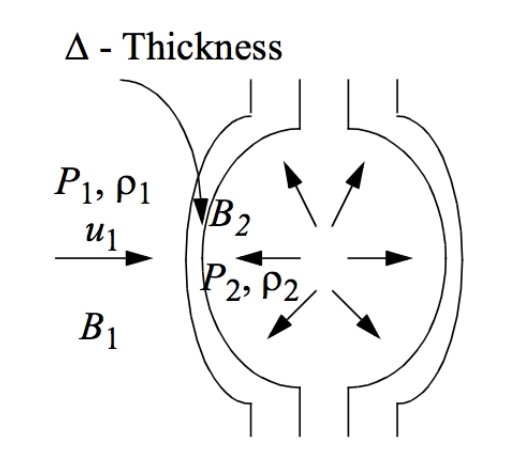
\includegraphics[width=0.3\textwidth]{hw5_p4.jpg} 
\end{center}
Conservation of momentum
(or sometimes called pressure balance) sets one of the jump conditions of the
forward shock
\begin{equation}
    P_1+\rho_1u_1^2+\frac{B_1^2}{2\mu_0}
    =P_2+\rho_2u_2^2+\frac{B_2^2}{2\mu_0}
\end{equation}

(a) The late-stage forward shock of a strongly-magnetized supernova shell
($\rho_2,P_2,u_2,$ and $B_2$) moves at high $M_s$ into a weaky-magnetized
interstellar medium ($\rho_1,P_1,u_1,$ and $B_1$), having plowed the magnetic
field into a shell. Simplify the momentum equation by keeping only one dominant
term on each side of the equation. Explain why.

(b) Use magnetic flux conservation to derive a simple, geometric-based
relationship between the shell thickness ($\Delta$), the radius of the shell
($R$), $B_1$, and $B_2$.

(c) Combine the results above to derive a relation between the relative shell
thickness ($\Delta / R$) and the Alfvén Mach speed. If the ISM is weakly
magnetized, do we expect thin ($\Delta /R\ll1$) or thick ($\Delta /R\sim 1$)
shells? Explain. 
\begin{solution}
(a) Since $M_s\gg 1$, $\rho u^2\gg P$. The flow dominates the pressure
term. So both $P_1$ and $P_2$ can be neglected. Since the shell is highly
magnetized, the magnetic field term dominates. The opposite occurs in the ISM.
So then we can write
\begin{equation}\label{p4:pressure}
    \rho_1u_1^2=\frac{B_2^2}{2\mu_0} 
\end{equation}

(b) Assuming the shell is spherical, the magnetic flux of the ISM through it is 
just $\Phi_\text{ISM}=\pi R^2B_1$, since a sphere has a cross-sectional area of
$\pi R^2$. However, inside the thickness $\Delta$ of the shell, the cross
section is $2\pi R\Delta$. So the flux of the magnetic field inside the
shell is $2\pi R\Delta B_2$. Then by conservation of the magnetic flux,
\begin{equation}\label{p4:flux}
    \pi R^2B_1=2\pi R\Delta B_2\Rightarrow\frac{B_2}{B_1}=\frac{R}{2\Delta} 
\end{equation}

(c) Now, the Alfvén Mach number is defined as
\begin{equation}
    M_A^2=\frac12\frac{\rho_1u_1^2}{B_1^2/2\mu_0}
    =\frac12\frac{B_2^2}{B_1^2}
    =\frac18\frac{R^2}{\Delta^2}
    \Rightarrow\frac{\Delta}{R}=\frac1{2\sqrt2 M_A}
\end{equation}
If the ISM is weakly magnetized, $M_A\gg 1$, so $\Delta /R\ll 1$. This is
because the electric field inside the shell accelerates ions to high enough
energy and the magnetic field ejects them out into the ISM. So the shell can't
be very thick.
\end{solution}
\end{problem}
%%%%%%%%%%%%%%%%%%%%%%%%%%%%%%%%%%%%%%%%%%%%%%%%%%%%%%%%%%%%%%%%%%%%%%%%%%%%%%%%
%%%%%%%%%%%%%%%%%%%%%%%%%%%%%%%%%%%%%%%%%%%%%%%%%%%%%%%%%%%%%%%%%%%%%%%%%%%%%%%%
\begin{problem}{5}[Energy in Magnetic Reconnection]
Derive a simple expression for energy conservation in magnetic reconnection.
Justify the approximations that are made.

(a) The incoming energy flux can be written as
\begin{equation}\label{p5a:e_in}
    u_{\text{in}}\qty(\frac{\rho_{\text{in}}
    u_{\text{in}}^2}{2}+\frac{\gamma}{\gamma-1}P_\text{in}+\frac{B_{\text{in}}^2}{\mu_0}) 
\end{equation}
where $\vb{B}_\text{in}$ is the component parallel to the incoming surface.
Write a similar expression for the out-going energy flux. Derive an approximate
expression balancing the incoming and out-going energy flux given a diffusion
region size as indicated above.

(b) Use the continuity equation to show that $\Delta
\rho_{\text{in}}u_{\text{in}}=\delta\rho_{\text{out}}u_{\text{out}}$.

(c) Show that if $u_{\text{in}}\ll V_A$ then the kinetic energy of the inflow,
$u_{\text{in}}(1 /2\rho_{\text{in}}u_{\text{in}}^2)$, can be neglected.

(d) Argue from a geometric standpoint or by using $\div{\vb{B}}=0$ that
\begin{equation}
    \abs{\frac{B_{\text{out}}}{B_{\text{in}}}}\approx\frac\delta\Delta 
\end{equation}
so that the out-going magnetic energy is negligible (no need to be overly
rigorous).

(e) Show that the above equation reduces to
\begin{equation}
    \frac{B_{\text{in}}^2}{\mu_0\rho_{\text{in}}}+\frac{\gamma}{\gamma-1}\frac{P_{\text{in}}}{\rho_{\text{in}}}\approx\frac{u_{\text{out}}^2}{2}+\frac{\gamma}{\gamma-1}\frac{P_{\text{out}}}{\rho_{\text{out}}}  
\end{equation}

(f) Through observation and through kinetic analysis, one can demonstrate that
the outflow velocity is often at the Alfvén speed. If one ignores the
contribution of the pressure terms, is the energy equation balanced? If not,
what can you conclude about the temperatures or pressures of the inflow versus
the outflow.
\begin{solution}
(a) From \eqref{p5a:e_in}, the out-going energy flux is
\begin{equation}
    u_{\text{out}}\qty(\frac{\rho_{\text{out}}u_{\text{out}}^2}{2}
    +\frac{\gamma}{\gamma-1}P_{\text{out}}+\frac{B_{\text{out}}^2}{\mu_0})    
\end{equation}
Let us use the general expression in \eqref{p3:general},
$\div{\vb{\bm\Phi_\text{total}}}=0$ where $\bm\Phi_\text{total}$ is the energy
density flux of both the particles and the electromagnetic field. By Gauss
theorem,
\begin{equation}
    \int \div{\bm\Phi_\text{total}}d^3x=\oint \bm\Phi_\text{total}\vdot d\vb{A}=0 
\end{equation}
where the final equality assumes that the energy transport only happens between
the particles and the field.
\begin{center}
    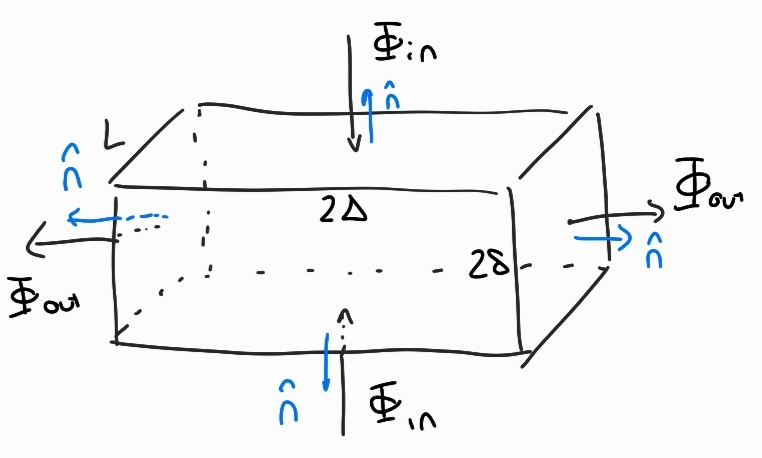
\includegraphics[width=0.5\textwidth]{hw5_p5.jpg} 
\end{center}
Since the dimensions of the reconnection site are
small enough that $\bm\Phi_\text{in}$ and $\bm\Phi_\text{out}$ are constant on
the surface (see the figure above), the surface integral is approximately
\begin{align}
    \oint\bm\Phi_\text{total}\vdot d\vb{A}
    \approx-2\Phi_\text{in} 2\Delta L+2\Phi_\text{out} 2\delta L=0
\end{align}
So we can relate the incoming and out-going energy flux as
\begin{equation}\label{p5a:energy}
    \Delta u_\text{in}
    \qty(\frac{\rho_\text{in}u_\text{in}^2}{2}+\frac{\gamma}{\gamma-1}P_\text{in}+\frac{B_\text{in}^2}{\mu_0})
    =
    \delta u_\text{out}
    \qty(\frac{\rho_\text{out}u_\text{out}^2}{2}+\frac{\gamma}{\gamma-1}P_\text{out}+\frac{B_\text{out}^2}{\mu_0})
\end{equation}

(b) Similar to the arguments in part (a), the continuity equation states that
$\div{\qty(\rho\vb{u})}=0$. So we can integrate on the surface of the
reconnection site
\begin{equation}
    \oint\qty(\rho\vb{u})\vdot d\vb{A}
    \approx-4\rho_\text{in}u_\text{in}+4\delta\rho_\text{out}u_\text{out}
    =0\Rightarrow\Delta\rho_\text{in}u_\text{in}=\delta\rho_\text{out}u_\text{out}
\end{equation}

(c) Factoring out $\rho_\text{in}$ in the LHS of \eqref{p5a:energy}, we get
\begin{equation}
    \Delta\rho_\text{in}u_\text{in}\qty(\frac{u_\text{in}^2}{2}+\frac{\gamma}{\gamma-1}\frac{P_\text{in}}{\rho_\text{in}}+V_A^2)
    \approx
    \Delta\rho_\text{in}u_\text{in}\qty(\frac{\gamma}{\gamma-1}\frac{P_\text{in}}{\rho_\text{in}}+V_A^2)
\end{equation}
if $u_\text{in}\ll V_A$.

(d) Since $\vb{B}_\text{in}$ is perpendicular to the normal vector of the upper
and lower surface in the Figure in part (a) and similarly for
$\vb{B}_\text{out}$, when evaluating the surface integral, we get
\begin{equation}
    \oint\div{\vb{B}}\vdot d\vb{A}\approx-4\delta B_\text{in}+4\Delta B_\text{out}=0 
    \Rightarrow\abs{\frac{B_\text{out}}{B_\text{in}}}=\frac\delta\Delta
\end{equation}

(e) Part (b) makes the pre-factors in \eqref{p5a:energy} cancel. Part
(c) and (d) make the terms $u_\text{in}$ and $B_\text{out}^2$ vanish.
So combining these results, \eqref{p5a:energy} reduces to
\begin{equation}
    \frac{\gamma}{\gamma-1}\frac{P_\text{in}}{\rho_\text{in}}
    +\frac{B_\text{in}^2}{\mu_0\rho_text{in}}\approx\frac{u_\text{out}^2}{2}+\frac{\gamma}{\gamma-1}\frac{P_\text{out}}{\rho_\text{out}}
\end{equation}

(f) Ignoring the pressure terms, we get a non-sensical result that
$u_\text{out}^2=2V_A^2\neq V_A^2$. Thus, using ideal gas law $P=nT$, we can
write
\begin{equation}
    \frac{\gamma}{\gamma-1}\qty(T_\text{out}-T_\text{in})=\frac{mV_A^2}2 
    \Rightarrow T_\text{out}-T_\text{in}=\frac{\gamma-1}{\gamma}\frac{mV_A^2}{2}
\end{equation}
\end{solution}
\end{problem}
%%%%%%%%%%%%%%%%%%%%%%%%%%%%%%%%%%%%%%%%%%%%%%%%%%%%%%%%%%%%%%%%%%%%%%%%%%%%%%%%
\end{document}
